\documentclass{beamer}

\mode<presentation> {
\usetheme{Boadilla}
}

\input{mycommands.sty}

\usepackage{graphicx} % Allows including images
\usepackage{booktabs} % Allows the use of \toprule, \midrule and \bottomrule in tables
\usepackage[T1]{fontenc}
\usepackage[utf8]{inputenc}
%\usepackage[french]{babel}
\usepackage{amsmath, amsthm, amssymb}

\definecolor{GreenTitle}{RGB}{141, 216, 141}
\definecolor{GreenBody}{RGB}{217, 242, 217}
\definecolor{GreenTitleFont}{RGB}{50, 100, 0}
\renewenvironment{definition}[1]{
\setbeamercolor{block body}{bg=GreenBody}
\setbeamercolor{block title}{fg=GreenTitleFont, bg=GreenTitle}
\begin{block}{#1}}
{\end{block}}

\definecolor{YellowTitle}{RGB}{255,221,77}
\definecolor{YellowBody}{RGB}{255,243,128}
\definecolor{YellowTitleFont}{RGB}{77,64,9}
\newenvironment{assumption}[1]{
\setbeamercolor{block body}{bg=YellowBody}
\setbeamercolor{block title}{fg=YellowTitleFont, bg=YellowTitle}
\begin{block}{#1}}
{\end{block}}


\title[HNF]{Hamiltonian Neural Flows\footnote{\href{https://arxiv.org/abs/1909.13789}{Hamiltonian Generative Networks}, Thoth \textit{et al.}}}

\author[Gaspard B.]{Gaspard Beugnot}
\date{March 17th, 2020}

\begin{document}

\begin{frame}
\titlepage
\end{frame}

\begin{frame}{Introduction}
\begin{itemize}
    \item À partir d'une séquence vidéo, apprendre l'Hamiltonien d'un système
    \begin{itemize}
        \item État = position + variable latente 
        \item Position = image
        \item Permet déroulement temporel en avant, en arrière, accéléré
    \end{itemize}
    \item Adapté au problème d'évaluation de densité:
    \begin{itemize}
        \item État = échantillon + variable latente
        \item Entraînement sur des échantillons tirés d'une loi
        \item Permet de transformer une loi simple en une loi complexe (Variational Inference with Normalizing Flows)
    \end{itemize}
\end{itemize}

Implémentation sur: \href{https://github.com/gaspardbe/HamiltonianGenerativeNetworks}{github.com/gaspardbe/HamiltonianGenerativeNetworks}.
\end{frame}

\begin{frame}{État de l'art}
\section{État de l'art}
\tableofcontents[currentsection]
\end{frame}

\begin{frame}{Inférence variationnelle}
\subsection{Inférence Variationelle}
\begin{itemize}
\item Décomposition variables observées / variables latentes 
\item Approximer la postérieure des variables latentes par une fonction paramétrique
\item Utiliser Jensen, optimiser l'approximation de la postérieure
\end{itemize}

\begin{center}
\begin{align*}
\log p_\theta (\bx) &= \log \int_\mathcal{Z} p_\theta (\bx | \bz) p(\bz) \dd z \\
&= \log \int\mathcal{Z} \frac{q_{\phi}(\bz | \bx)}{q_{\phi}(\bz | \bx)} p_\theta (\bx | \bz) p(\bz) \dd z \\
&\geq - \mathbb{D}_{KL} \csb{q_\phi (\bz | \bx) | p(\bz)} + \mathbb{E}_q \csb{\log p_\theta(\bx | \bz)} \\ 
&= \mathcal{F}(\bx)
\end{align*}
\end{center}

($\theta$: paramètres du modèle; $\phi$: paramètres du réseau)
\end{frame}

\begin{frame}{Normalizing Flows (Rezende \textit{et al.})}
\subsection{Normalizing Flows}
\begin{itemize}
    \item<1-> A priori: $\pi( \cdot )$
    \item<2-> Fonction inversible $f(\cdot)$
    \item<3-> Loi objectif: $p(\boldsymbol{x}) = \pi\p{f^{-1}(x)} \left\lvert \det{\frac{\partial f^{-1}}{\partial \boldsymbol{x}}} \right\rvert$
\end{itemize}

\onslide<4-> Problème: comment calculer le Jacobien efficacement?
\end{frame}

\begin{frame}{Variational inference with Normalizing Flows}
\begin{itemize}
\item<1-> Planar Flows
\begin{itemize}
\item Transformation de type: 
\begin{equation*}
f( \bz ) = \bz + \boldsymbol{u} h (\boldsymbol{w}^\top \bz +b)
\end{equation*} 
\item Ensemble de contractions dilatations orthogonalement à $\boldsymbol{w}$.
\item Déterminant calculable en temps linéaire par rapport au nombre de dimensions.
\end{itemize}
\item<2-> Radial flows
\begin{itemize}
\item Transformation de type: 
\begin{equation*}
f(\bz) = \bz + \beta \frac{\bz - \bz_0}{\alpha + \left\lVert \bz - \bz_0 \right\rVert}
\end{equation*}
\item Contraction radiale par rapport à un point de référence $\bz_0$. 
\item Déterminant calculable en temps linéaire à nouveau.
\end{itemize}
\end{itemize}
\end{frame}

\begin{frame}{Expressivité}
Des flots qui restent expressifs (gaussienne en distribution initiale). 
\begin{center}
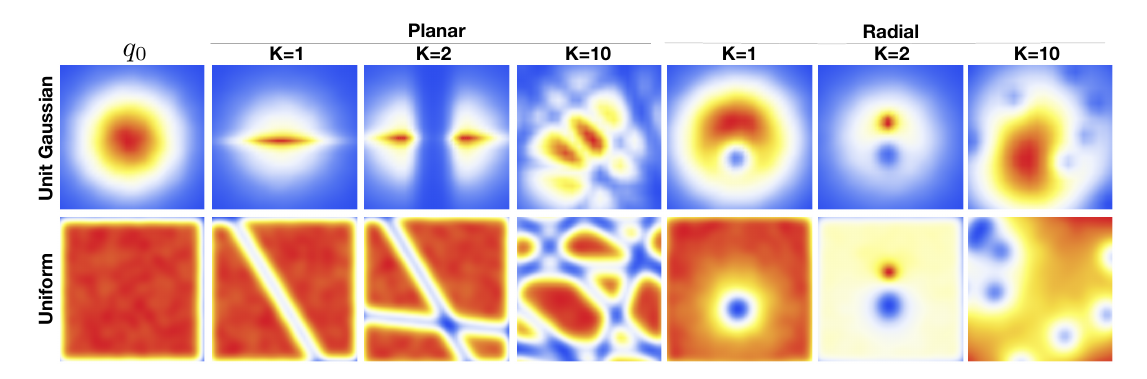
\includegraphics[width=.9\linewidth]{samples/normalizing_flows_expressivity.png}
\end{center}
\end{frame}

\begin{frame}{Hamiltonian Monte Carlo}
\subsection{Hamiltonian Monte Carlo}
\onslide<1->Principe (Neal) 
\begin{itemize}
\item MCMC = générer une chaîne de Markov avec loi a posteriori pour loi invariante 
\item Énergie : 
\begin{equation*}
H(q, p) = \frac{1}{Z} \exp{\p{-U(q)}} \exp{\p{-K(p)}}
\end{equation*}
avec $U(q) = - \log\p{\pi(q) p(q | \theta)}$. 
\item Si $K(p) \varpropto p^\top M p$, $\iff$ $p$ variable latente tirée suivant une gaussienne. 
\end{itemize}

\onslide<2->Résultats: 
\begin{itemize}
\item déplacements sur des isodensités pour $H$, peut explorer différents modes pour $q$.
\item Réversibilité du Hamiltonien donne automatiquement la \textit{detailed balance equation}.
\item Nécessite de choisir judicieusement les paramètres d'intégration. 
\end{itemize}
\end{frame}

\begin{frame}{HMC with NN}
\subsection{HMC avec NN}
Principe (Levy): 
\begin{itemize}
\item Utiliser des opérateurs d'échelles sur la mise à jour des états (translations, dilatation sur l'état et sur le gradient).
\item Coût doit:
\begin{itemize}
\item maximiser le mixing (maximise la taille des sauts, ie. distance entre les états) 
\item encourage un burn-in rapide (atteindre l'état stationnaire rapidement)
\end{itemize}
\item Convergence vers la loi invariante garantie par la réversibilité
\end{itemize}
\end{frame}

\begin{frame}{Schémas numériques pour l'intégration - Euler}
\subsection{Schémas numériques}
\centering
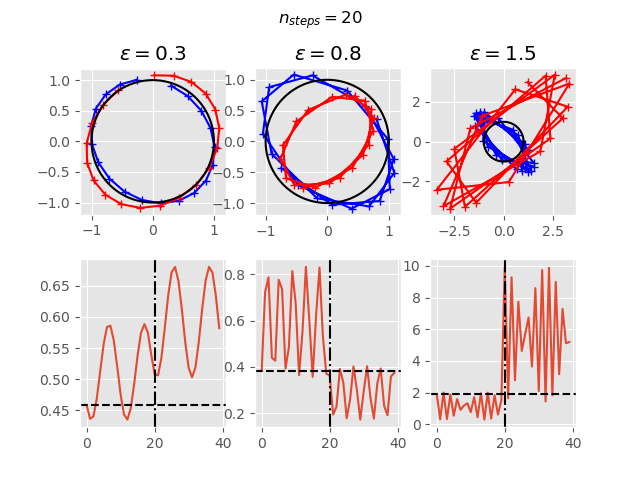
\includegraphics[width=.9\linewidth]{samples/euler_example.png}
\end{frame}

\begin{frame}{Schémas numériques pour l'intégration - Leapfrog}
\centering
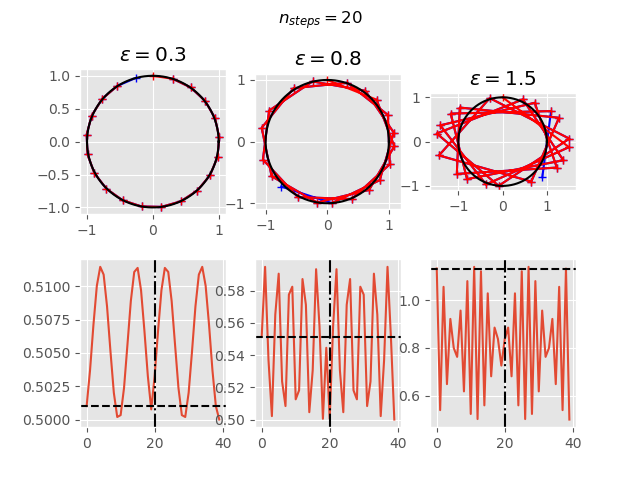
\includegraphics[width=.9\linewidth]{samples/leapfrog_example.png}
\end{frame}

\begin{frame}{Neural Hamiltonian Flow}
Principe: 
\begin{itemize}
\item Utiliser $T$ hamiltoniens pour modéliser un flot qui emmène d'un a priori simple à une fonction complexe.
\begin{itemize}
\item \textbf{Préserve le volume} : pas de déterminant à calculer
\item \textbf{Réflexif} : inverse naturel et facile à calculer 
\end{itemize}
\item État = $\bs_0, ..., \bs_T$ avec $\bs_i = \bq_i, \bp_i$. Moment = \textbf{variable latente}: 
\begin{align*}
p(\bq_T) &= \int p(\bq_T, \bp_T) \dd \bp_T \\
&= \int \pi(\HH_1^{-\dd t} \circ \dots \circ \HH_T^{-\dd t} (\bq_T, \bp_T)) \dd \bp_T
\end{align*}
\end{itemize}
Impossible d'explorer tout l'espace des $\bp$ : $\to$ encoder le moment depuis la position. 
\end{frame}

\begin{frame}{ELBO}
On approche la probabilité par une fonction paramétrique:

\begin{align*}
\log p(\bq_T) &= \log \int p(\bq_T, \bp_T) \ \dd\bp_T \\
    &= \log \int \frac{p(\bq_T, \bp_T)}{f_{\psi}(\bp_T | \bq_T)} f_{\psi}(\bp_T | \bq_T) \ d\bp_T \\
    &\geq  \mathbb{E}_{f_{\psi}(\bp_T | \bq_T)}[\log \ \pi ( \mathcal{H}_1^{-dt} \circ \ldots \circ \mathcal{H}_T^{-dt}(\bq_T, \bp_T) )  \\
    & - \log \ f_{\psi}(\bp_T | \bq_T)\ ] \\
    &= \text{ELBO}(\bq_T)
\end{align*}

On optimise cette borne inf par rapport à $\psi$ et les $T$ hamiltoniens.
\end{frame}

\begin{frame}{Détails Techniques}
Plusieurs modules: 
\begin{itemize}
\item Hamiltonien:
\begin{itemize}
\item 2 réseaux de neurones (MLP): $U(\bq)$ (potentiel) et $K(\bp)$ cinétique
\item Une fonction d'intégration: $\bq, \bp \mapsto \bq', \bp'$.
\end{itemize}
\item Un encodeur:
\begin{itemize}
\item 2 réseaux de neurones (MLP): $\boldsymbol{\mu}, \boldsymbol{\sigma} : \RR^d \to \RR^d$.
\item Échantillonne selon une gaussienne de loi $\boldsymbol{\mu}, \boldsymbol{\sigma}$.
\end{itemize}
\item Le flot: 
\begin{itemize}
\item Définit une a priori
\item Implémente les fonctions de coûts 
\item Optimise les paramètres par rétropropagation.
\end{itemize}
\end{itemize}
\end{frame}

\begin{frame}{Objectif}
\begin{center}
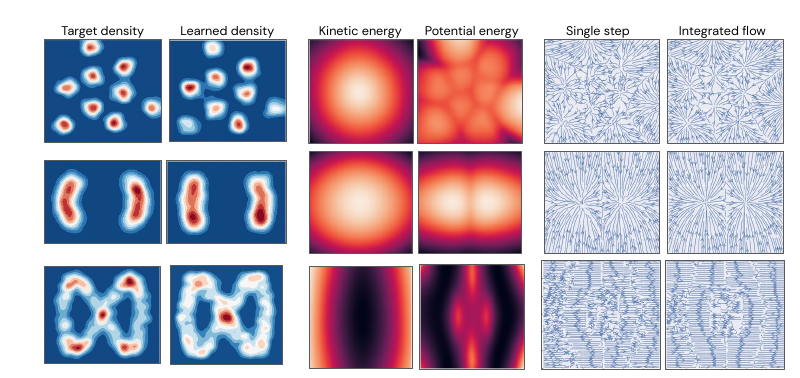
\includegraphics[width=\linewidth]{samples/objective.png}
\end{center}

\end{frame}

\begin{frame}{Résultats numériques}
Instabilités numériques...
\centering
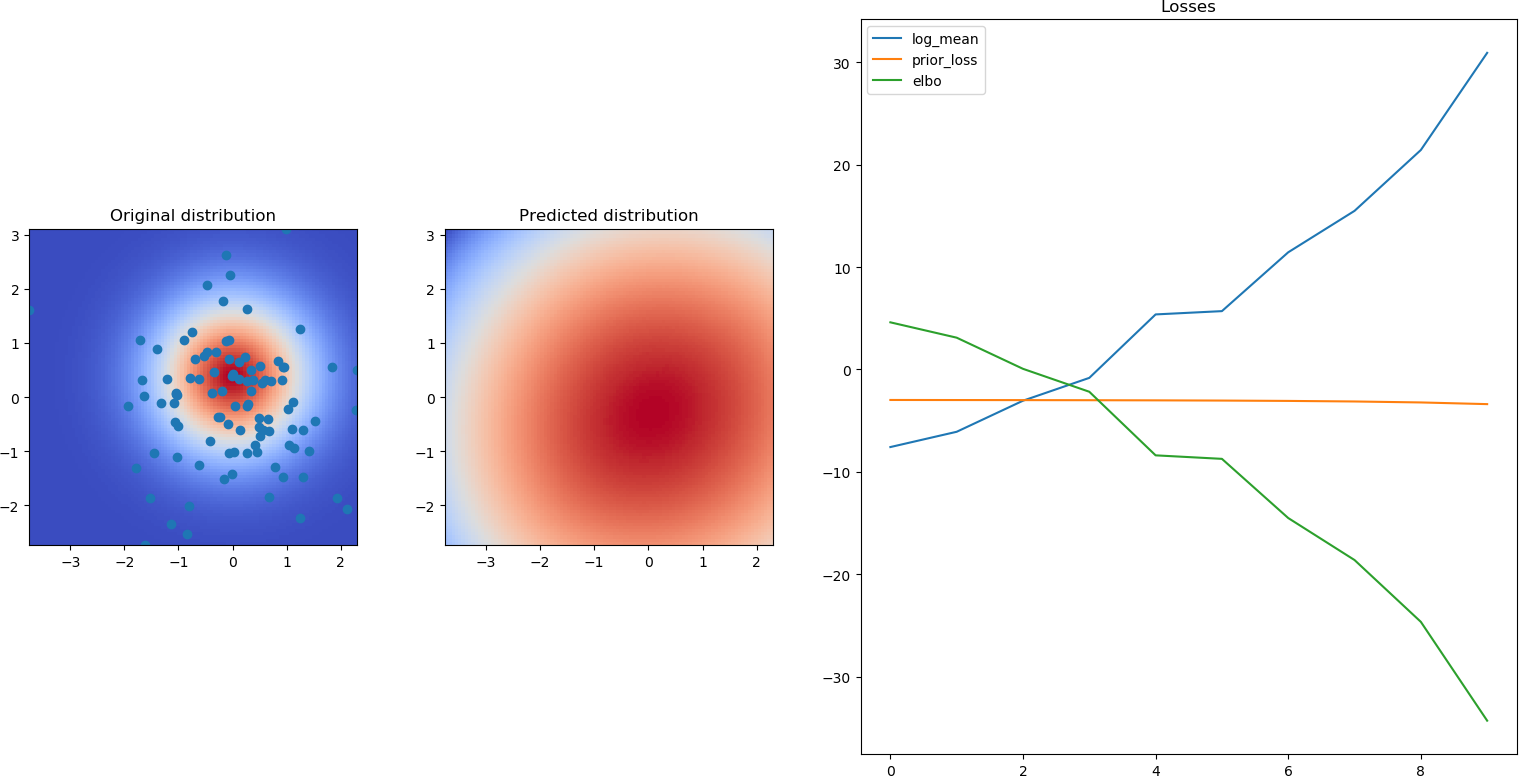
\includegraphics[width=\linewidth]{samples/gaussian_failed.png}
\end{frame}

\begin{frame}{Prolongements}
Beaucoup de questions en suspend: 
\begin{itemize}
\item Quelle est l'utilité de plusieurs hamiltoniens vs. 1 hamiltonien complexe?
\item Comment procéder à l'échantillonnage ? \emph{First, we assume that the initial state $s_0$ is a sample from a simple prior $s_0 \sim \pi_0 (\cdot)$}.
\begin{itemize}
\item On ne peut pas explorer tout l'espace des moments
\item Entraîner un \textbf{nouvel} encodeur ?
\end{itemize}
\item Notion de dynamique: 
\begin{itemize}
\item Peu de pas d'intégration...
\item Interprétation simple $\implies$ overkill? Échantillons = bassin d'attraction?
\end{itemize}
\end{itemize}

\end{frame}

\end{document}
